\documentclass{beamer}
\graphicspath{ {graphics/}}

\begin{document}
\title{Literary Worlds Javascript Client}
\author{John Lewis, Owen Watson, Tim Cunningham}
\usenavigationsymbolstemplate{}
\frame{\titlepage}
\frame{\frametitle{Table of contents}\tableofcontents}

\section{Background}
\frame{\frametitle{Background}
\begin{itemize}
  \item Literary Worlds is an multiuser text based game used for English education at WMU.
  \item These games are known as MOOs (Multiuser Object Oriented), or MUDs (Multi User Domains)
  \item Most of these games provide a telnet interface for playing, Literary Worlds uses enCore with MOOtcan, a Java applet.
  \item The aim of this project is to provide a drop-in replacement user interface in Javascript.
\end{itemize}
}

\frame{\frametitle{enCore Xpress interface}
  \begin{centering}
  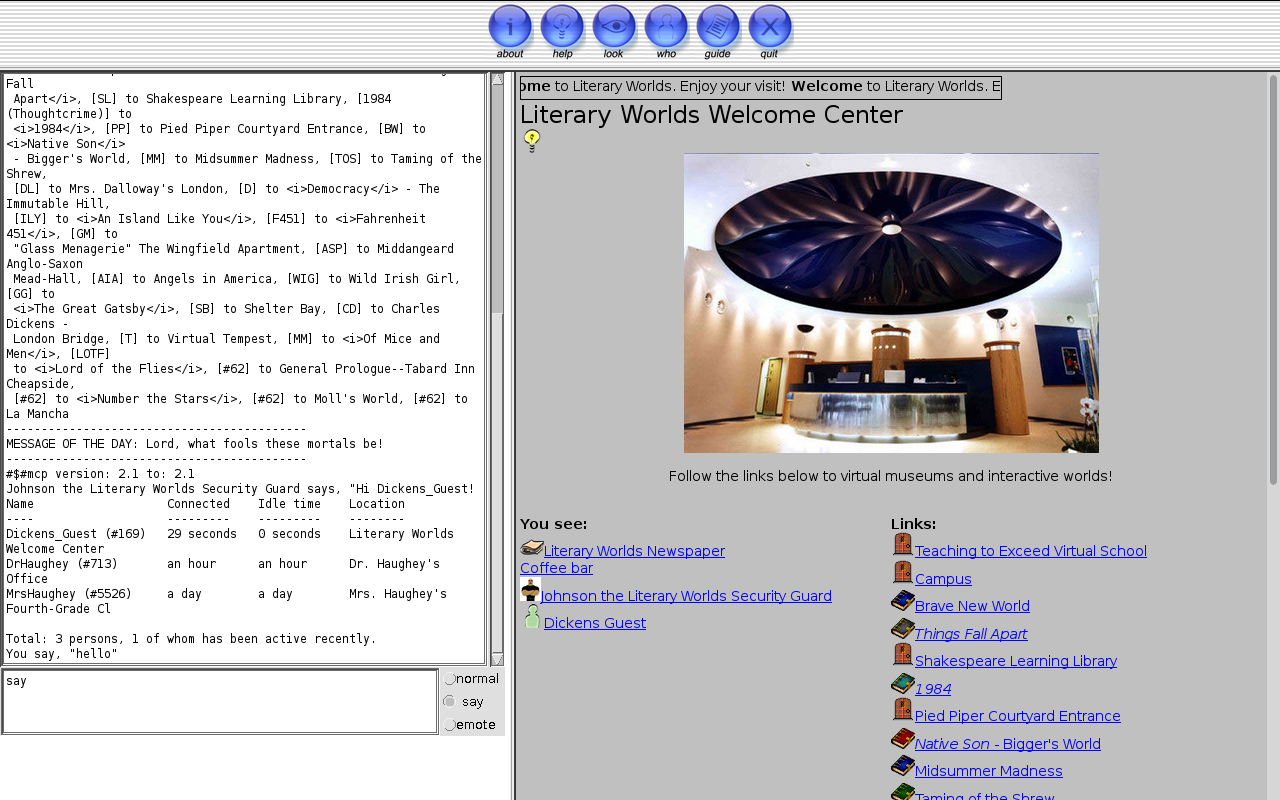
\includegraphics[width=\textwidth,height=\textheight,keepaspectratio]{classUsage.png}
  \end{centering}
}

\frame{\frametitle{Client}
\begin{itemize}
  \item Client: Allen Webb
  \item Professor of Comparative Literature and Postcolonial Studies at Western Michigan University's Department of English
  \item In 2003, Robert Rozema, a PhD student under Allen Webb created the prototype Literary World.
  \item Several virtual worlds were created that form the Literary Worlds project.
  \item The Literary Worlds project was one of seven projects to receive funding from the Western Michigan University President's Innovation Fund.
\end{itemize}
}

% - Title Page
% - Abstract
% - TOC
% - Intro
% - Background
% - Design Decisions
% - Stories
% - Implementation
%   - Continuous Integration - Tim
% - Testing
%   - Owen
% - Security
%   - Telnet is insecure
%   - Contain telnet in docker or similar
% - References
% - Glossary

\section{Introduction}
\frame{\frametitle{Technical Introduction}
  \begin{itemize}
    \item LambdaMOO is a MUD server software package(as well as a particular MUD), Literary Worlds uses the server software.
    %\item LambdaMOO is distributed as a source tarball, deploying it on a new sever entails compiling it, and running it using the enCore database, and configuring Apache to work with enCore.
    \item enCore Xpress is an graphical interface and MUD database package that works with the LambdaMOO server to provide a browser based text client using a Java applet as well as a graphical, mouse driven interface.
    %\item The Java applet is the text interface, it makes a telnet to LambdaMOO, as though the user were using a command line telnet client.
    \item Literary Worlds uses version 4 of enCore, there is a version 5 of enCore that attempts to provide a web interface without a Java applet, however it is beta software and hasn't been actively developed since 2006.
  \end{itemize}
}

\frame{\frametitle{Plugin Missing}
  \begin{centering}
  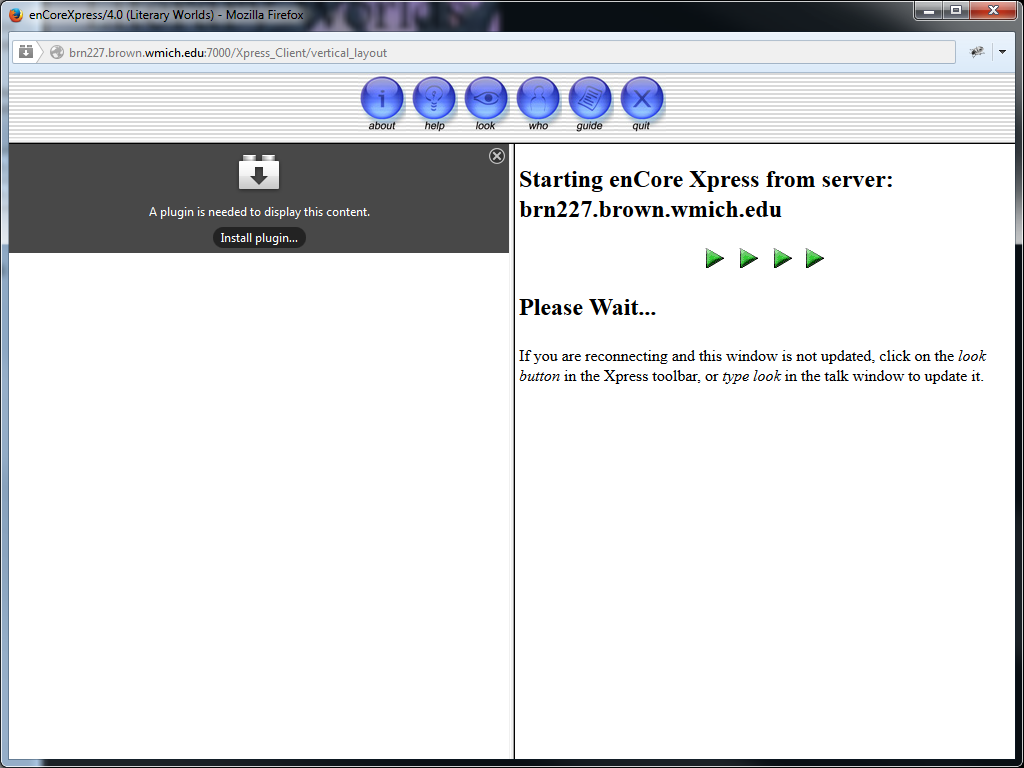
\includegraphics[width=\textwidth,height=\textheight,keepaspectratio]{PlugInNeeded.png}
  \end{centering}
}

\frame{\frametitle{Client-Server Diagram}
  \begin{centering}
  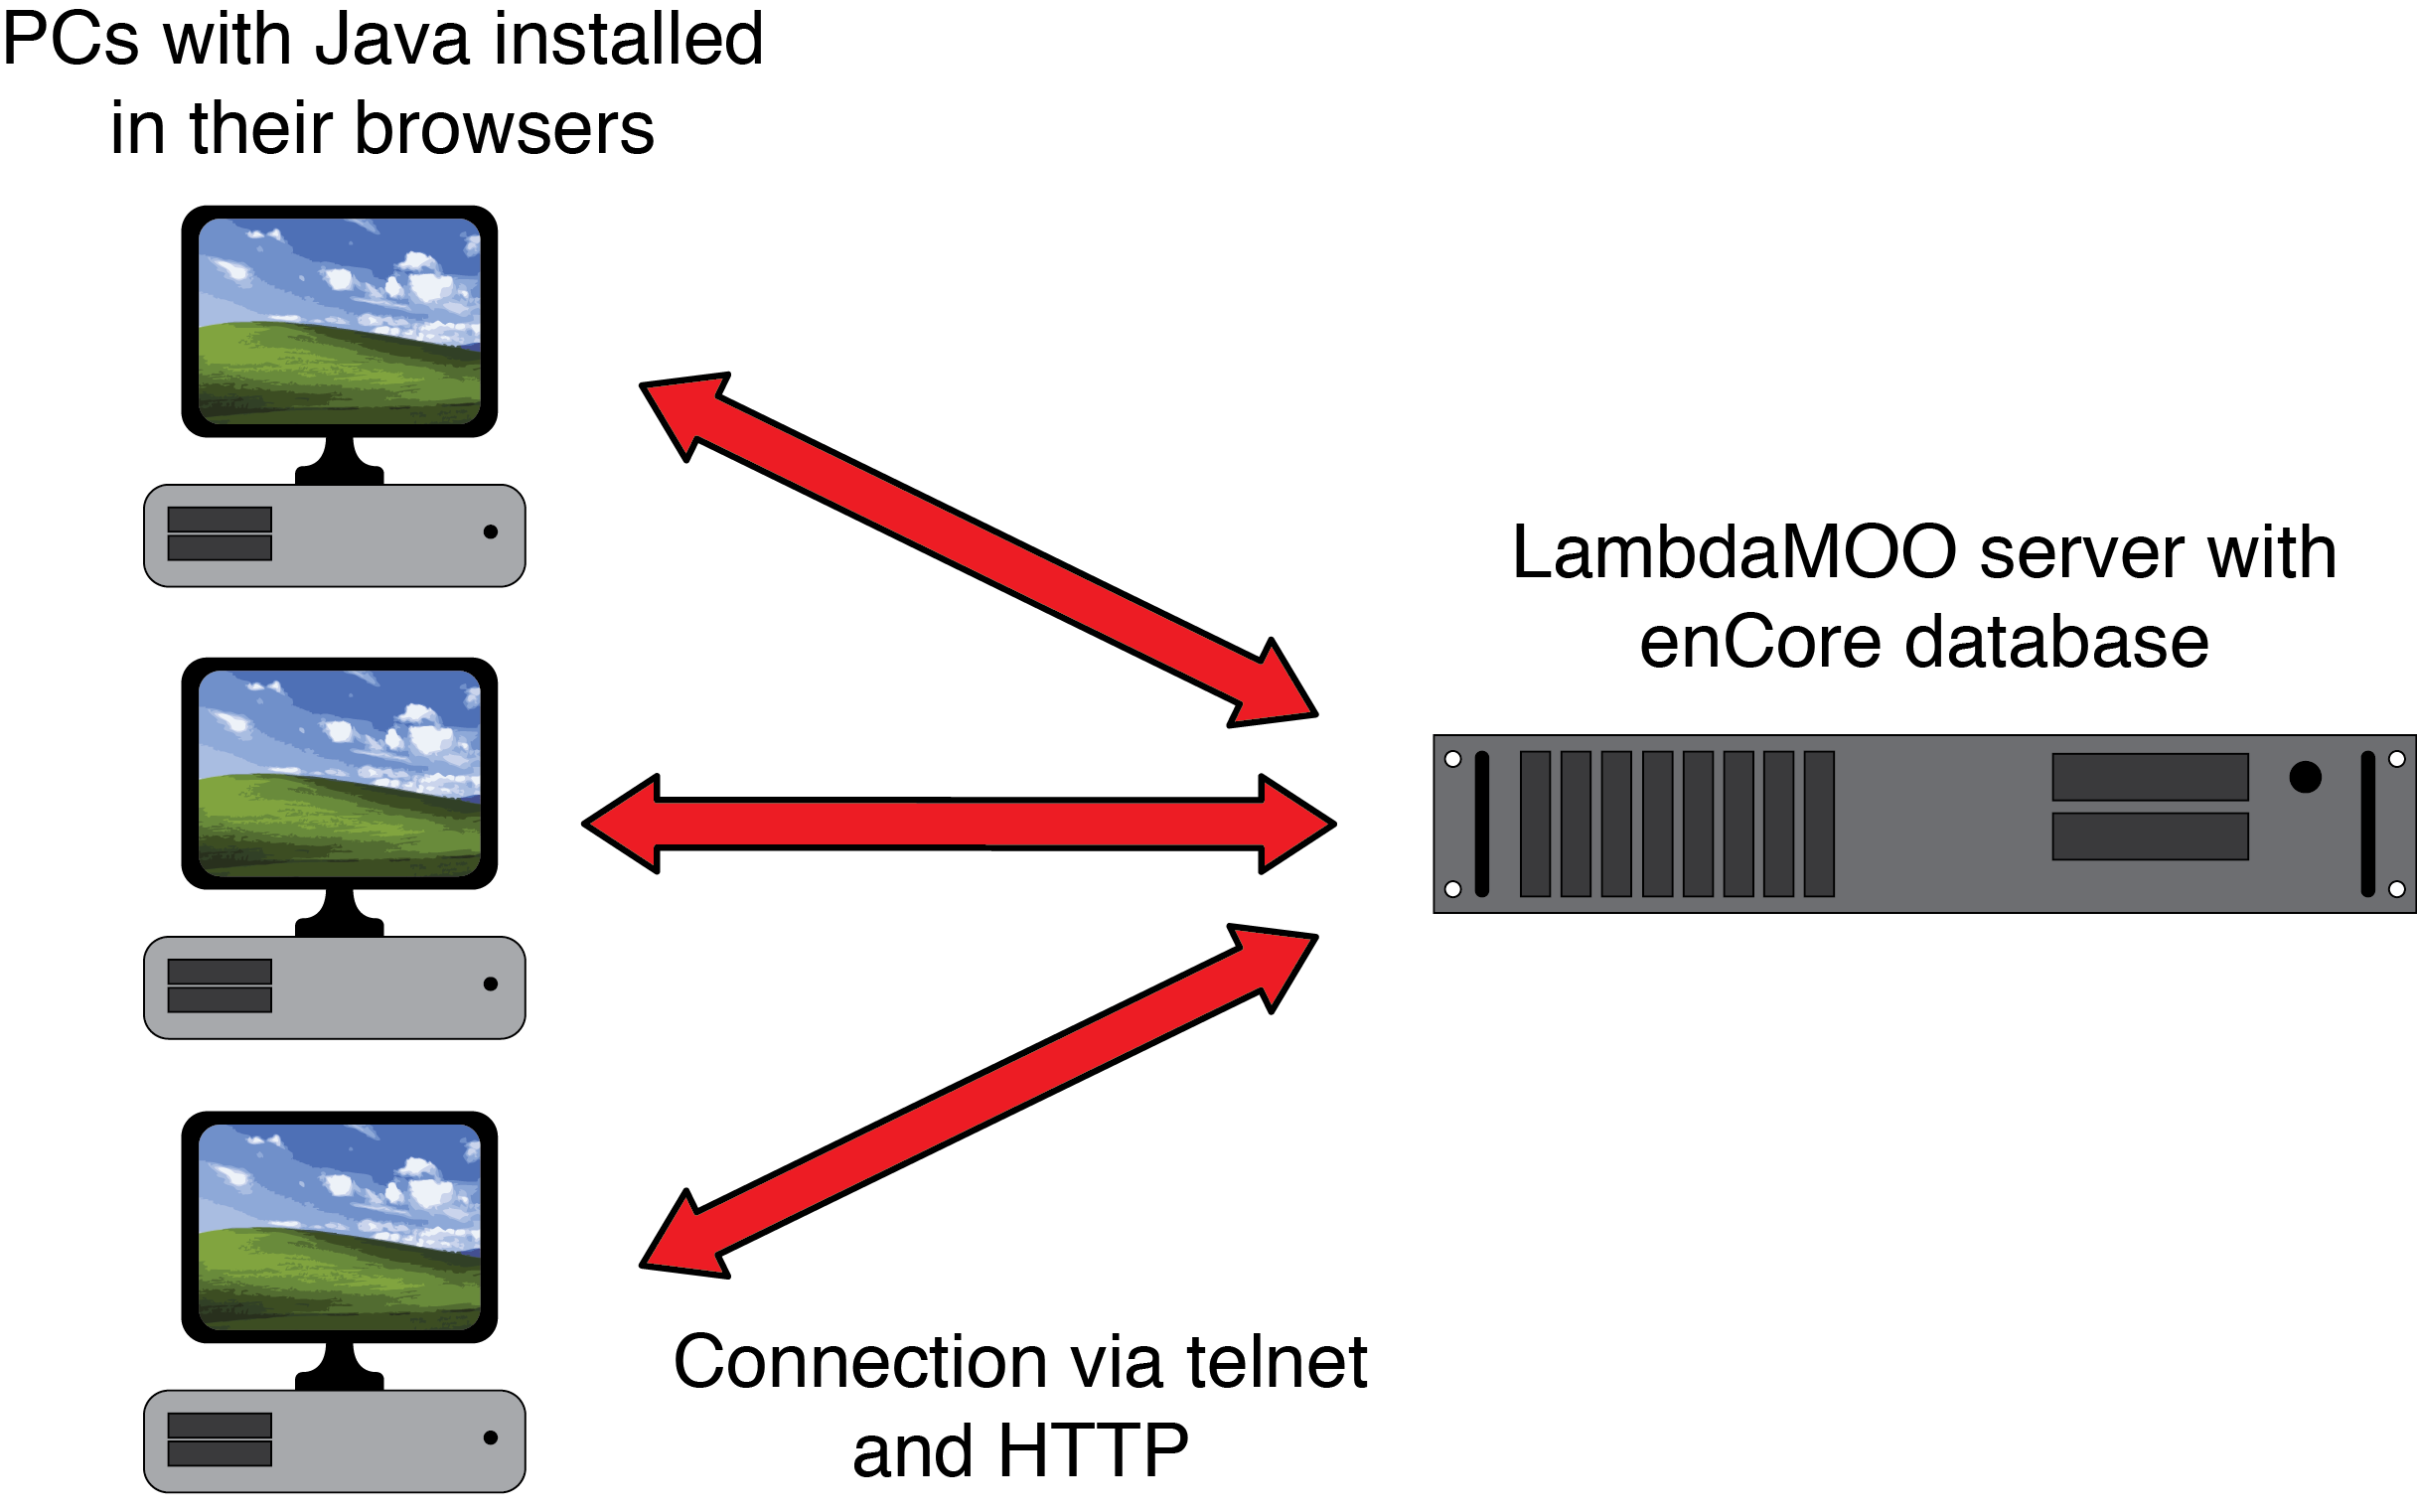
\includegraphics[width=\textwidth,height=\textheight,keepaspectratio]{TelnetDiagram.png}
  \end{centering}
}

\section{Design Decisions}
\frame{\frametitle{Client-Server Design}
  \begin{itemize}
    \item It is not possible to initiate a raw TCP connection in clientside Javascript, unlike Java applets.

    \item Therefore, we need an intermediary server to connect over TCP, as well as to the browser client, and send data back and forth between the two.

    \item This server must also support multiple concurrent users and handle asynchronous tasks and events.
  \end{itemize}
}

\frame{\frametitle{Client-Server Diagram}
  \begin{centering}
  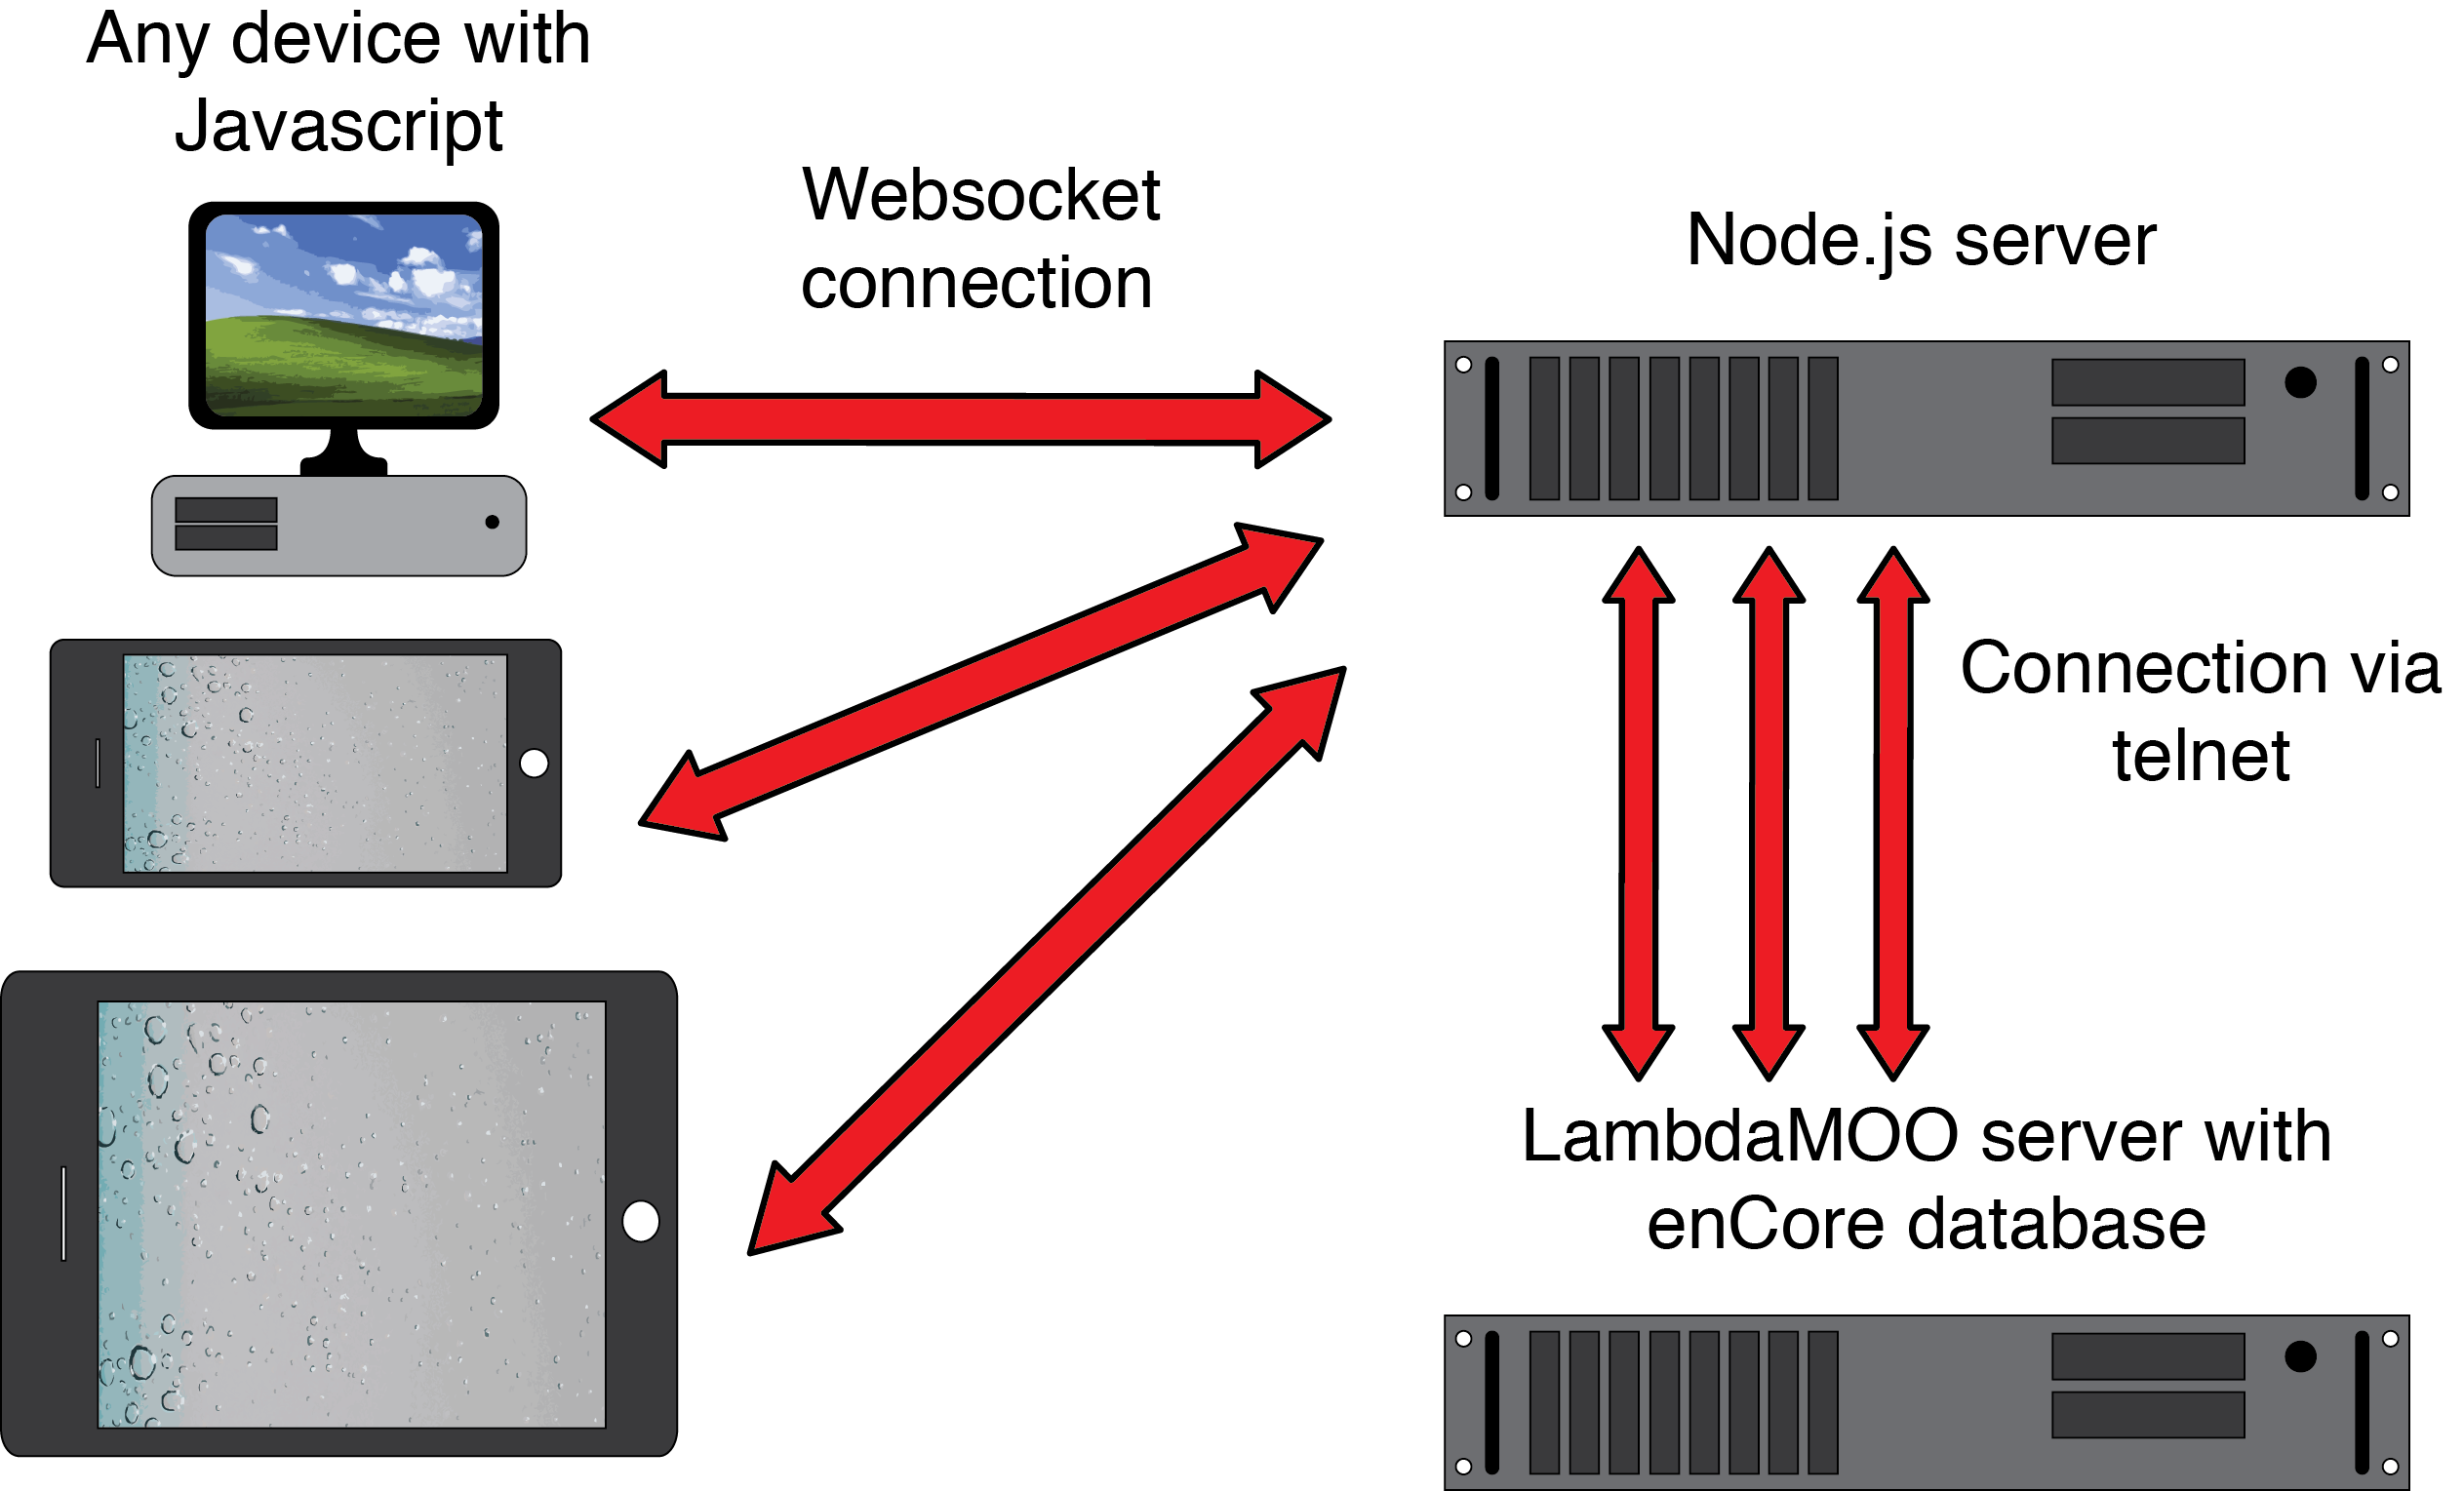
\includegraphics[width=\textwidth,height=\textheight,keepaspectratio]{NodeDiagram.png}
  \end{centering}
}

\frame{\frametitle{Client Technology}
  % Backbone, Bootstrap, Socket.io, Coffeescript
  \begin{itemize}
  \item Socket.io
    \begin{itemize}
      \item Allows realtime communication between a server program and browser clients.
    \end{itemize}
  \item Backbone
    \begin{itemize}
      \item Backbone is a templating library for Javascript web applications
    \end{itemize}
  \item Bootstrap
    \begin{itemize}
    \item Bootstrap is a frontend layout toolkit
    \end{itemize}
  \item Coffeescript
    \begin{itemize}
      \item Coffeescript is a simple language that translates to Javascript
    \end{itemize}
  \end{itemize}
}

\frame{\frametitle{Basic Text Interface}
  \begin{centering}
  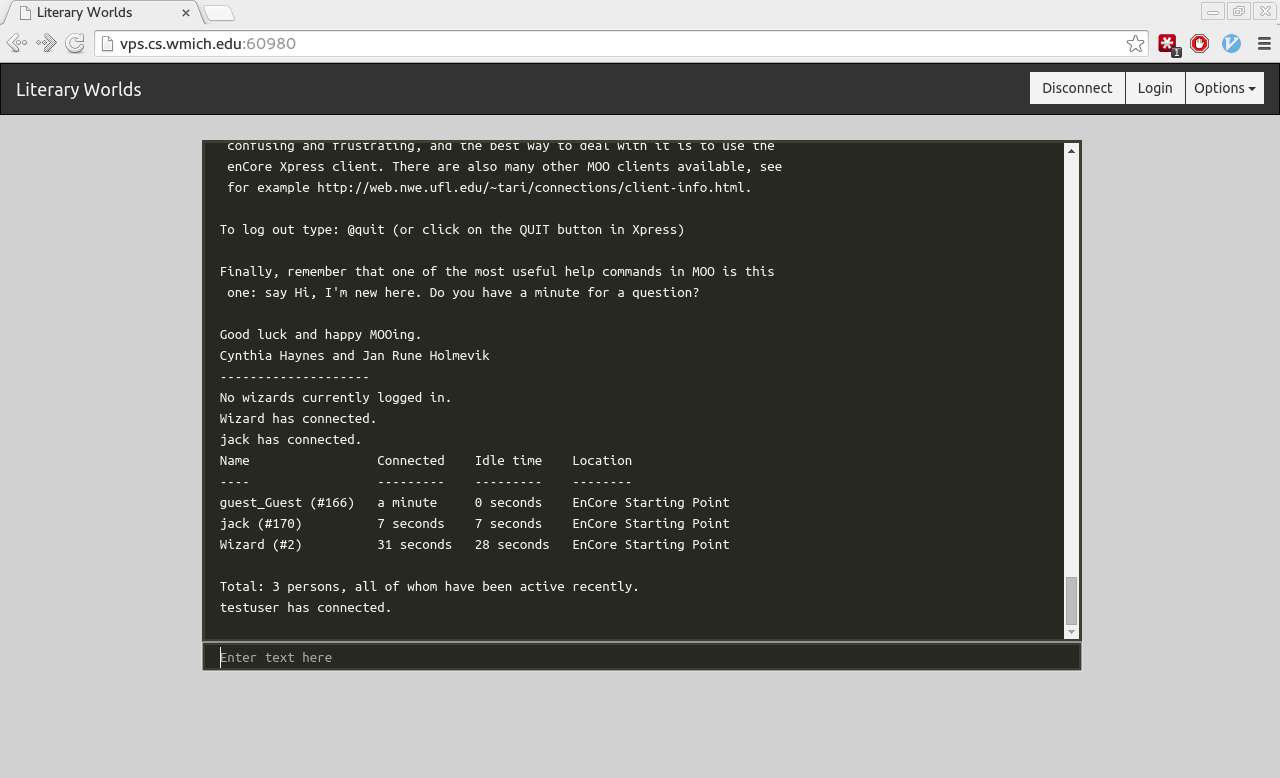
\includegraphics[width=\textwidth,height=\textheight,keepaspectratio]{litworlds.png}
  \end{centering}
}
\frame{\frametitle{Server Technology}
  % Node.JS here
  \begin{itemize}
  \item Node.js
    \begin{itemize}
      \item Node.js is a server side runtime that uses the asynchronous features of Javascript to build web application servers. It provides a rich set of networking libraries, and uses the Google Chrome Javascript engine, V8.
      \item It is the first class citizen for socket.io, so it was natural to choose it for the server.
    \end{itemize}
  \item Express
    \begin{itemize}
      \item Express is a web app framework for Node.js
      \item In provides tools such as easy interfaces for REST, URL routing, cookies, etc. similar to what Ruby on Rails does for the Ruby language.
    \end{itemize}
    \item Socket.io
  \end{itemize}
}


\section{Stories}
\frame{\frametitle{Stories}
  \begin{itemize}
  \item Text Mode
    \begin{itemize}
      \item Client side Javascript MUD client
      \item This is reason an intermediary server is needed, to handle the telnet connection on behalf of each client.
    \end{itemize}
  \item Graphical Mode
    \begin{itemize}
      \item This work is already done in enCore Xpress, there is no need to reinvent it.
      \item The new web application will simply need to serve the existing enCore Xpress interface in a coherent way.
    \end{itemize}
  \end{itemize}
}

\section{Implementation}
\frame{\frametitle{Continuous Integration}
\begin{itemize}
  \item Purpose
  \begin{itemize}
    \item Continuous integration aims to merge code from a developer's working copy many times a day into a shared mainline.
    \item Before any code is merged a, build server runs unit tests on the code, and if passed will be merged into the mainline.f
    \item This helps to improve the quality of the software and reduce the time to deliver it.
    \item The end goal of this process is to be able to automatically build and deploy the software whenever all of the tests are passing
  \end{itemize}
  \item Possible Tools
  \begin{itemize}
  	\item Jenkins
  	\item CICircle
	\item TeamCity
	\item Hudson
  \end{itemize}
\end{itemize}
}

\frame{\frametitle{Jenkins}
  \begin{itemize}
    \item Pros:
    \begin{itemize}
      \item Widely used and documented
      \item open sourced
      \item Wide range of support for different systems
      \item Can be extended with plugins
      \item Github integration
    \end{itemize}
    \item Cons:
    \begin{itemize}
      \item Manual setup required
      \item Have to get a server to run Jenkins
    \end{itemize}
  \end{itemize}
}

\section{Testing}
\frame{\frametitle{Unit Testing}
  \begin{itemize}
    \item Framework
    \item Matching Tools
  \end{itemize}
}

\section{Security}
\frame{\frametitle{Security}
  \begin{itemize}
    \item Telnet is plain text in transport, so it is inherently vulnerable to eavesdropping.
    \item For the initial work on the project, security is not a main concern.
    \item In the future, the telnet server can be protected from external network connections using containerization such as docker
    \item This way only the Node.js server can connect via telnet, and user data can be protected with SSL in transport.
    \item This strategy would disable the legacy enCore Xpress interface
  \end{itemize}
}

\end{document}
